% !TeX root = ../thuthesis-example.tex

\chapter{引言}

自从上世纪50年代人工智能概念提出以来,自然语言处理(NLP)经历了从基于规则到统计方法,再到机器学习的演变。早期的规则系统和统计模型虽然取得了一定进展,但受限于语言复杂性和数据规模,效果有限。直到2010年代,深度学习的兴起为NLP带来了突破,尤其是2018年Transformer模型~\cite{Vaswani+2017}的提出,彻底改变了这一领域。基于Transformer的预训练语言模型(如BERT~\cite{devlin2018bert}、GPT~\cite{radford2018improving}系列)通过海量数据训练,在文本理解、生成和翻译等任务上表现出色,显著提升了机器处理自然语言的能力。 


预训练语言模型范式主要包含两个阶段。第一个阶段是在大量无标注语料上进行大规模预训练,目标是构建一个能力足够通用且强大的基础模型(Foundation Model)。这一阶段的预训练使模型能够学习到语言的通用特征和知识,为后续任务打下坚实基础。第二阶段则是在下游任务上进行微调,即针对使用者特别关注的领域,对基础模型进行该领域的继续训练,从而构建更精准的分支模型。这种两阶段范式显著提升了模型的泛化能力以及在多样化任务上的适应性和性能。

近年来,随着扩展定律(Scaling Law)的发现~\cite{kaplan2020scaling},构建越来越大的模型成为公司和机构共同追求的目标。更大的模型规模通常意味着更强的能力,尤其是在复杂任务上展现出惊人的潜力。然而,这些大模型的训练过程成本高昂,可能对资源造成很大的浪费。因此,如何在提升模型性能的同时实现对资源的高效利用,已成为当前人工智能领域亟待解决的重要问题。本文在预训练——微调范式下,面向扩展定律所导致的大语言模型,遵循提高预训练可预测性、降低微调资源开销的总体思路,对大模型进行了全流程的训练效率改进。

本章将为读者介绍本文的研究背景,探讨预训练——微调范式下两阶段各自面临的训练效率挑战,并且详细阐明本文的研究内容和主要贡献。


\section{研究背景}

自然语言处理的发展历程本质上反映了人类对语言认知规律的探索深化与计算范式革新之间的双重变奏。1950年艾伦·图灵提出“模仿游戏”测试时,符号主义学派主导着早期NLP研究,诺姆·乔姆斯基的生成语法体系试图通过形式化规则解析语言结构。然而这种基于演绎逻辑的方法在面对自然语言的歧义性和语境依赖性时遭遇根本性困境,正如1966年ALPAC报告~\cite{ALPAC}所指出的,单纯依靠人工编写语法规则难以实现真正的语言理解。

统计语言模型的兴起标志着NLP进入数据驱动的新阶段。1980年代隐马尔可夫模型在语音识别中的成功应用,1990年代最大熵模型和条件随机场在词性标注等序列标注任务中的突破,逐渐确立了概率图模型的主导地位。这一时期的里程碑式进展背后,是香农信息论与贝叶斯统计的深度融合,语言处理开始被视为概率空间中的最优推断问题。然而,传统统计方法严重依赖特征工程,其浅层模型架构难以捕捉语言的多层次抽象特性。

深度学习的革命性突破始于2013年词向量(Word2vec)技术~\cite{mikolov2013efficient}的出现,通过分布式表示实现了语义空间的连续映射。长短时记忆网络(LSTM)~\cite{hochreiter1997long}在机器翻译等任务中展现出的序列建模能力,使得神经网络开始全面取代统计模型。但真正引发范式转换的是2017年Transformer架构~\cite{Vaswani+2017}的提出——其自注意力机制突破了RNN的序列计算瓶颈,使并行化训练超长文本序列成为可能。2018年BERT~\cite{devlin2018bert}模型首次验证了预训练-微调范式的有效性,通过掩码语言建模(MLM)任务使模型学习到深层次的语境化表示,由此开启了大规模预训练语言模型的时代。

% 这一“预训练-微调”技术演进背后蕴含着深刻的神经科学启示。大脑皮层的层次化信息处理机制为深度神经网络提供了生物学基础,赫布理论(Hebbian Theory)关于"神经元同步激活则连接增强"的学说,与自监督预训练中的权重更新机制形成跨学科呼应。特别是预测编码理论(Predictive Coding)指出,大脑通过不断预测感官输入来构建世界模型,这与语言模型基于上文预测下文的自回归机制具有惊人的相似性。这些认知科学的理论积淀,为当前预训练范式提供了超越工程实践层面的理论支撑。

当前大模型训练已进入百万亿参数时代,其资源消耗呈指数级增长趋势。OpenAI的GPT-4模型训练需要消耗约$10^{25}$ FLOPs运算量,更严峻的是,由于扩展定律揭示的性能与模型规模、数据量、计算量的幂律关系,追求更大规模模型成为必然选择。预训练是一项极为复杂的系统工程。训练过程涉及大量超参数的调整,模型训练还会出现不稳定情况,同时可能伴随涌现现象,这些都使得预训练的结果充满不确定性。要是盲目开展训练,最终成果很可能达不到预期,只能重新进行实验与训练,造成资源的大幅浪费。

在微调阶段,虽然所需计算量通常比预训练低很多个数量级,但面临更复杂的优化曲面。一方面,下游任务的多样性要求为每个任务保存独立的全参数模型副本,另一方面, 预训练模型蕴含的通用语言知识与特定任务需求之间存在复杂映射关系,仅仅基于梯度下降的微调过程不能拿有效利用预训练获得的先验能力,从而在样本利用效率上大打折扣。更实际的问题是,微调阶段资源的提供方通常只有非常少的算力,无法进行大数据,全参数的微调。因此少参微调成为了重要的手段,但是传统少参微调方法通常只能使用默认模块进行微调,这样可能会导致模型性能不能充分发挥,从而不能高效提升微调效率。





\section{研究意义}
大模型训练是大模型开发生命周期的关键环节,预训练质量决定大模型能力上限,微调效果影响其应用适配度。为提升大模型训练两阶段的效率,我们针对不同痛点,研究可预测预训练技术和低资源微调技术。以下从四个角度探讨本文高效训练方法的研究价值:

\begin{enumerate}
  \item 降低预训练成本与提升成功率。深度学习网络性能受网络架构、训练超参数等多种因素影响,传统研究常需大量调参实验确定最佳训练配置。进入预训练时代,大模型训练成本飙升。当前领先的预训练模型规模达千亿参数量、十万亿数据量(按词元统计),计算成本极高,且实验耗时久,迭代效率低。可预测预训练将目标网络性能转化为函数外插拟合问题,通过小规模模型快速迭代实验,经精细扩展定律拟合外推至大模型,变同规模大量参数搜索为小规模快速迭代,大幅降低实验成本。同时,大规模深度学习网络训练常遇不稳定、效果不佳问题,如损失突增、爆炸等。可预测预训练能提前预判此类问题,实现早干预、早调整,提升预训练成功率。
  \item 减少下游任务适配的数据与硬件需求。下游任务适配和预训练面临不同效率问题。下游任务需求由用户定义,传统微调虽无需预训练量级数据,但需专有领域万量级数据。本文研究的提示学习大幅减少数据需求,使预训练模型经零样本或少样本训练就能在下游任务取得良好性能。此外,下游任务使用者通常缺乏大模型预训练机构的大量计算和存储资源,即便依靠预训练机构微调,机构也难提供参数各异的任务特异模型。本文研究使不同任务资源需求降至普通全参数微调的万分之一,大幅降低计算资源。
  \item 增强对未来技术的预判能力。可预测预训练技术不仅能提高当前大模型训练效率,还能增强对未来技术的预判。大模型预训练核心是找到可扩展技术路线,不同路线扩展斜率不同。该技术让研究者更好预判特定技术路线下模型发展潜力,提前知晓技术上限和潜力。了解当前技术上限可催生新技术,知晓不同技术潜力能合理分配资源,有助于对未来技术发展做出更好决策。
  \item 促进大模型社区的多样性与繁荣。降低下游任务适配的数据和硬件需求,将使更多任务能以低门槛适配大模型,增加大模型社区多样性。即便使用同一基础模型,也会因适配数据和参数高效微调模块不同,展现差异化能力。同时,门槛降低会吸引更多行业成员活跃于大模型社区,创造更多分支模型,提升社区繁荣度。
\end{enumerate}


\section{研究内容与主要贡献}
本文所研究的高效性主要体现在两个阶段:(1)预训练阶段成本高昂,而大模型本身因为是一个复杂系统,会出现不稳定性以及伴生的涌现现象,导致预训练结果难以预期。如果盲目训练,很可能不及预期而需要重新实验和训练,导致资源成倍地浪费。(2)微调阶段目标多样模型庞大。目标多样主要是因为不同任务的数据分布不同,模型和任务的适配性也不同,因此通常需要为特定任务进行微调。而模型本身体积庞大,每次微调如果要收集大量特定数据,进行大算力训练,对造成模型应用上的困难。提示学习和参数高效微调是可以缓解这两个问题的方法,然而两种方法均仍然有大量改进空间。

具体而言, 本文设计了一套全流程的高效训练方案,在上述两个阶段进行创新。(1)预训练阶段,通过深入挖掘超参数扩展规律和性能扩展规律,构建可复用扩展定律与高效退火迭代技术,克服超参稳定性弱,性能涌现性强的问题和预测开销大,干预程度小的问题,使预训练变得更可预测,在预训练成本高昂的背景下提供精准的扩展定律。(2)微调阶段,通过运用能力激活与知识提示微调降低数据需求,克服提示微调数据利用效率低下的问题,通过实现模块自动化寻优与轻便框架降低存算需求,克服少参微调模块配置寻优困难的问题,使得目标多样模型庞大的微调阶段消耗资源大幅降低。下面简要介绍本文的主要贡献。

\begin{figure}
  \centering
  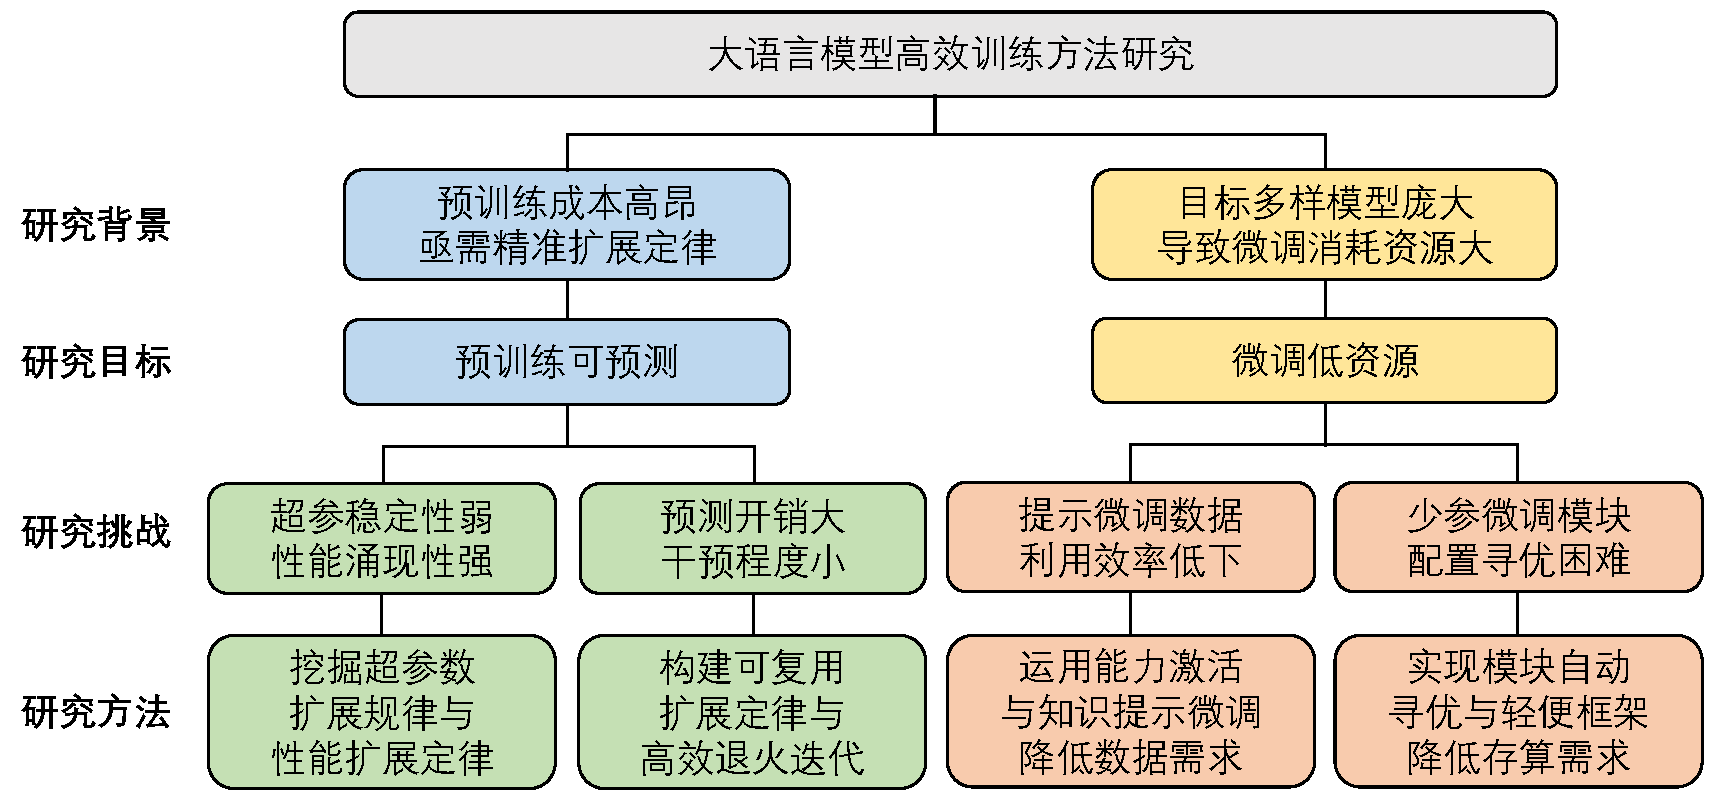
\includegraphics[width=\textwidth]{chap01/phdthesismain.pdf}
  \label{fig:mainframework}
  \caption{本文主要研究内容}
  \end{figure}

  
\subsection{可预测预训练之超参数扩展规律与性能扩展定律}
本研究首先基于Tensor Program~\cite{yang2022tensor}进行探索。Tensor Program中提出一种方法,希望通过对超参数的重参数化以及有理论保障的外推方法获得不随模型规模变化的稳定超参数。然而Tensor Program并未在实践上证明对于真实场景的模型训练的有效性。本文在真实场景对tensor program进行了深入研究,发现在辅以批量大小的扩展方案时,可以获得稳定的学习率扩展规律。本研究还对其他一些结构变体,例如QK-Norm,是否能对超参数稳定起到关键作用进行了研究。

在得到了稳定的超参扩展规律带来的损失扩展规律以后,本研究继续深入探索了性能扩展规律。性能扩展定律是一个非常困难的事情。这是因为一个任务的性能不仅影响因素众多,而且还会表现出波动性和涌现性(被称作涌现能力)。前人的研究主要集中在对涌现能力的定性研究,并且认为因为这种涌现能力的存在,导致任务性能是无法预测。针对这个问题,本研究进行了深入实验,提出一种基于大量采样的提升模型评估分辨率的方法,我们证明了这一方法是真实表现的无偏估计,并且假如计算资源允许,可以精确到任意精度。我们进一步提出了性能扩展定律,区别于损失扩展定律,该定律可以直接对下游任务性能进行预测。我们进一步引入了数据集级别扩展和样本级别扩展两种方案,并且提出损失辅助预测方法。这些方法将性能预测精度提升到99\%以上,初步解决了性能扩展规律的问题。

\subsection{可预测预训练之可复用扩展定律与高效退火迭代}
本研究首先分析了进行扩展定律拟合过程中的资源消耗,发现现有文献的拟合方法需要消耗的计算量和调研模型参数规模个数以及调研数据规模个数都成线性关系,因此在数据和模型两个维度的扩展定律研究需要消耗平方复杂度的算力。本研究思考了不同数据量下的模型训练无法复用训练过程的原因,将其归结为学习率调度对损失的影响带来的不可复用性。本研究分析了当前绝大部分模型训练都使用的学习率调度策略,提炼出其效果优异的原因,即同时具备全局最优解寻找和局部最优解寻找(退火)的特点。本研究提出将占训练过程绝大部分时间的全局最优解进行多模型共享,再通过时机各异的局部最优解寻找来完成模型训练。本研究证明,这种方法使数据维度的扩展定律拟合消耗的资源变为常数量级,有效提高了扩展定律拟合过程的高效性。

本研究进一步实验指出,基于以上策略的扩展定律拟合方法,由于其可复用的退火阶段,使得高质量数据迭代实验变得非常高效。本研究仔细研究了退火过程中引入不同数据对于模型训练结果的影响。发现在退火过程中引入高质量数据能显著提高模型在下游任务上的表现。由于可复用的退火阶段在整个训练过程占比很小,所以可以使用少量的算力进行多次性能迭代。除此之外,本研究还探索了退火迭代的训练动力学方面的原因,为后人对训练机理的探索~\cite{wen2024understanding}提供了新的方向。本研究综合利用上述方法,利用1/7的算力和1/3的模型大小,训练了性能超越Llama2-7B的模型,证明了本研究方案的有效性。

\subsection{少样本微调之能力激活与知识激活}
本研究从微调阶段的数据角度出发,首先研究了对于预训练模型对于分布外任务,是否可以使用少量数据习得。本文以一类名为“错误先验立场”的问题入手。该类问题的特点是回答该类问题的知识存在于大语言模型的预训练阶段,但是由于分布的差异导致模型无法有效调用这些知识进行回答。我们第一次提供了精标注的人类对于“错误先验立场”问题的回答,我们证明,只需要百到千量级的数据,就可以将模型的回复正确率从随机提升到接近90的准确率。这一发现提供了“小数据激活大能力”的有力证据,该思路也在后续的Instruction Tuning以及RLHF等工作中得到了进一步验证。

本研究进一步探索了对于与预训练模型能力更为接近的分布内任务,例如情感分类和主题分类,是否可以通过更少量的样本或者零样本来进行适配。知识微调是大模型范式下的有效适配手段,其利用模板和表达器来完成模型训练分布到任务输入输出空间的变换。本研究进一步提出了知识提示微调的概念,即在提示微调的基础上,引入知识库扩充的表达器,使得模型在微调过程中可以更好地利用预训练模型的知识。本研究指出通过在提示微调的表达器中引入人类知识先验,能够将模型性能提升高达17\%。

\subsection{少参数微调之模块自动化寻优与轻便代码框架}
本研究从微调阶段的存算资源角度出发,研究了少参数微调的自动化模块选择功能。传统少参微调的方法会选择默认模块进行微调。尽管这种方法能够大幅减少需要微调的参数量,然而由于在预训练过程中,不同模块已经训练出不同的分工,微调时使用默认模块可能会导致模型性能不能充分发挥。本研究提出了一种基于自动化模块选择的少参微调框架,该框架建立在对所有少参微调方法的统一建模视角下,借鉴了神经架构自动搜索算法(NAS),并创新地提出了可训练硬稀疏化优化目标,精准控制可微调参数总量。本研究使少参微调所需的微调参数量从全参数的1\%进一步降低到1\%\%量级,大幅减少了存算资源需求。

由于本研究构建于对所有少参微调方法的统一建模视角下,因此本研究也同时提供了一个灵活轻便的少参微调代码库:OpenDelta。区别于之前的代码库例如AdapterHub~\cite{pfeiffer2020adapterhub}, 本代码库在实现上通过“猴子补丁”的方式灵活修改预训练模型的张量流,使其能够动态加载和移除任意位置的少参微调模块,也可以同时加载多个少参微调模块,甚至组合不同种类的少参微调模块。在用户体验上,本代码库提供了一套完整的少参微调模块接口,用户可以通过简单的配置文件,即可实现对预训练模型的少参微调。



\section{本文组织结构}
本文共分为七章,其中第一章(即本章)为引言,主要介绍了本文的研究背景、研究意义、研究内容和主要贡献。第二章为相关工作,主要介绍了与本文研究内容相关的国内外研究现状和发展动态。第三章为预训练阶段的高效训练方法的第一部分,主要介绍超参数扩展规律和性能扩展规律,第四章为预训练节段的高效训练方法的第二部分,主要介绍可复用扩展定律和高效退火迭代。第五章为微调阶段的高效方法第一部分,主要介绍了能力激活与知识提示微调。第六章为微调阶段的高效训练方法,主要介绍了模块自动化寻优与轻便的少参微调框架。第七章为总结与展望,主要总结了本文的研究工作,并对未来的研究方向进行了展望。

